% \begin{frame}{Issue? How to show multiplicity?}
%     \begin{table}[h!]
%         \centering
%         \small
%         \begin{tabular}{|c|c|c|}
%         \hline
%         t\_pdg\_parent  & AL9       & SL7       \\ \hline
%         -11             & 2         & 0         \\
%         0               & 2         & 0         \\
%         22              & 2610      & 2397      \\
%         32              & 115877    & 112809    \\ \hline
%         \end{tabular}
%         \caption{Count of t\_pdg\_parent}
%         \label{table:truth_efficiency}
%         All particles are daughters of the Dark Photon? 
%     \end{table}
%     \begin{figure}
%         \begin{subfigure}[t]{0.35\linewidth}
%             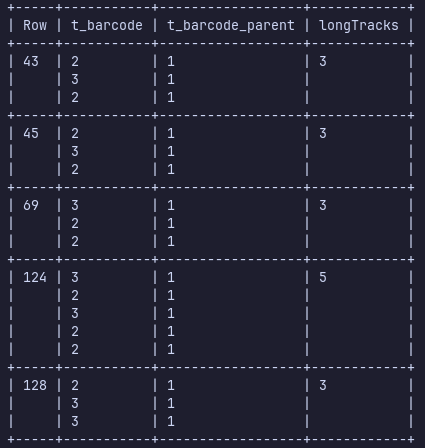
\includegraphics[width=\linewidth]{assets/Duplicates_tbarcode.png}            
%         \end{subfigure}
%         \begin{subfigure}[t]{0.35\linewidth}
%             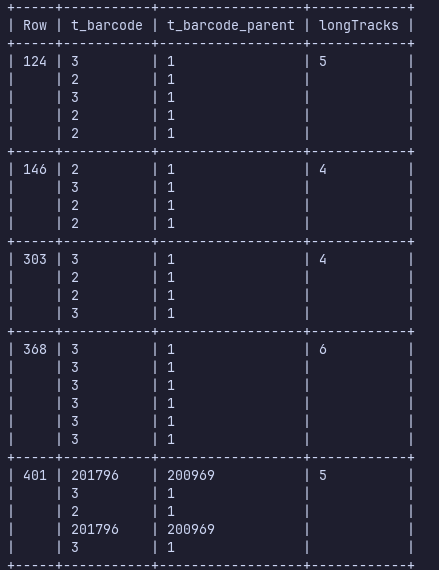
\includegraphics[width=\linewidth]{assets/Duplicates_tbarcode2.png}            
%         \end{subfigure}
%     \end{figure}
% \end{frame}


% \begin{frame}{Duplicate Tracks ? [Delete]}
%     \begin{figure}
%         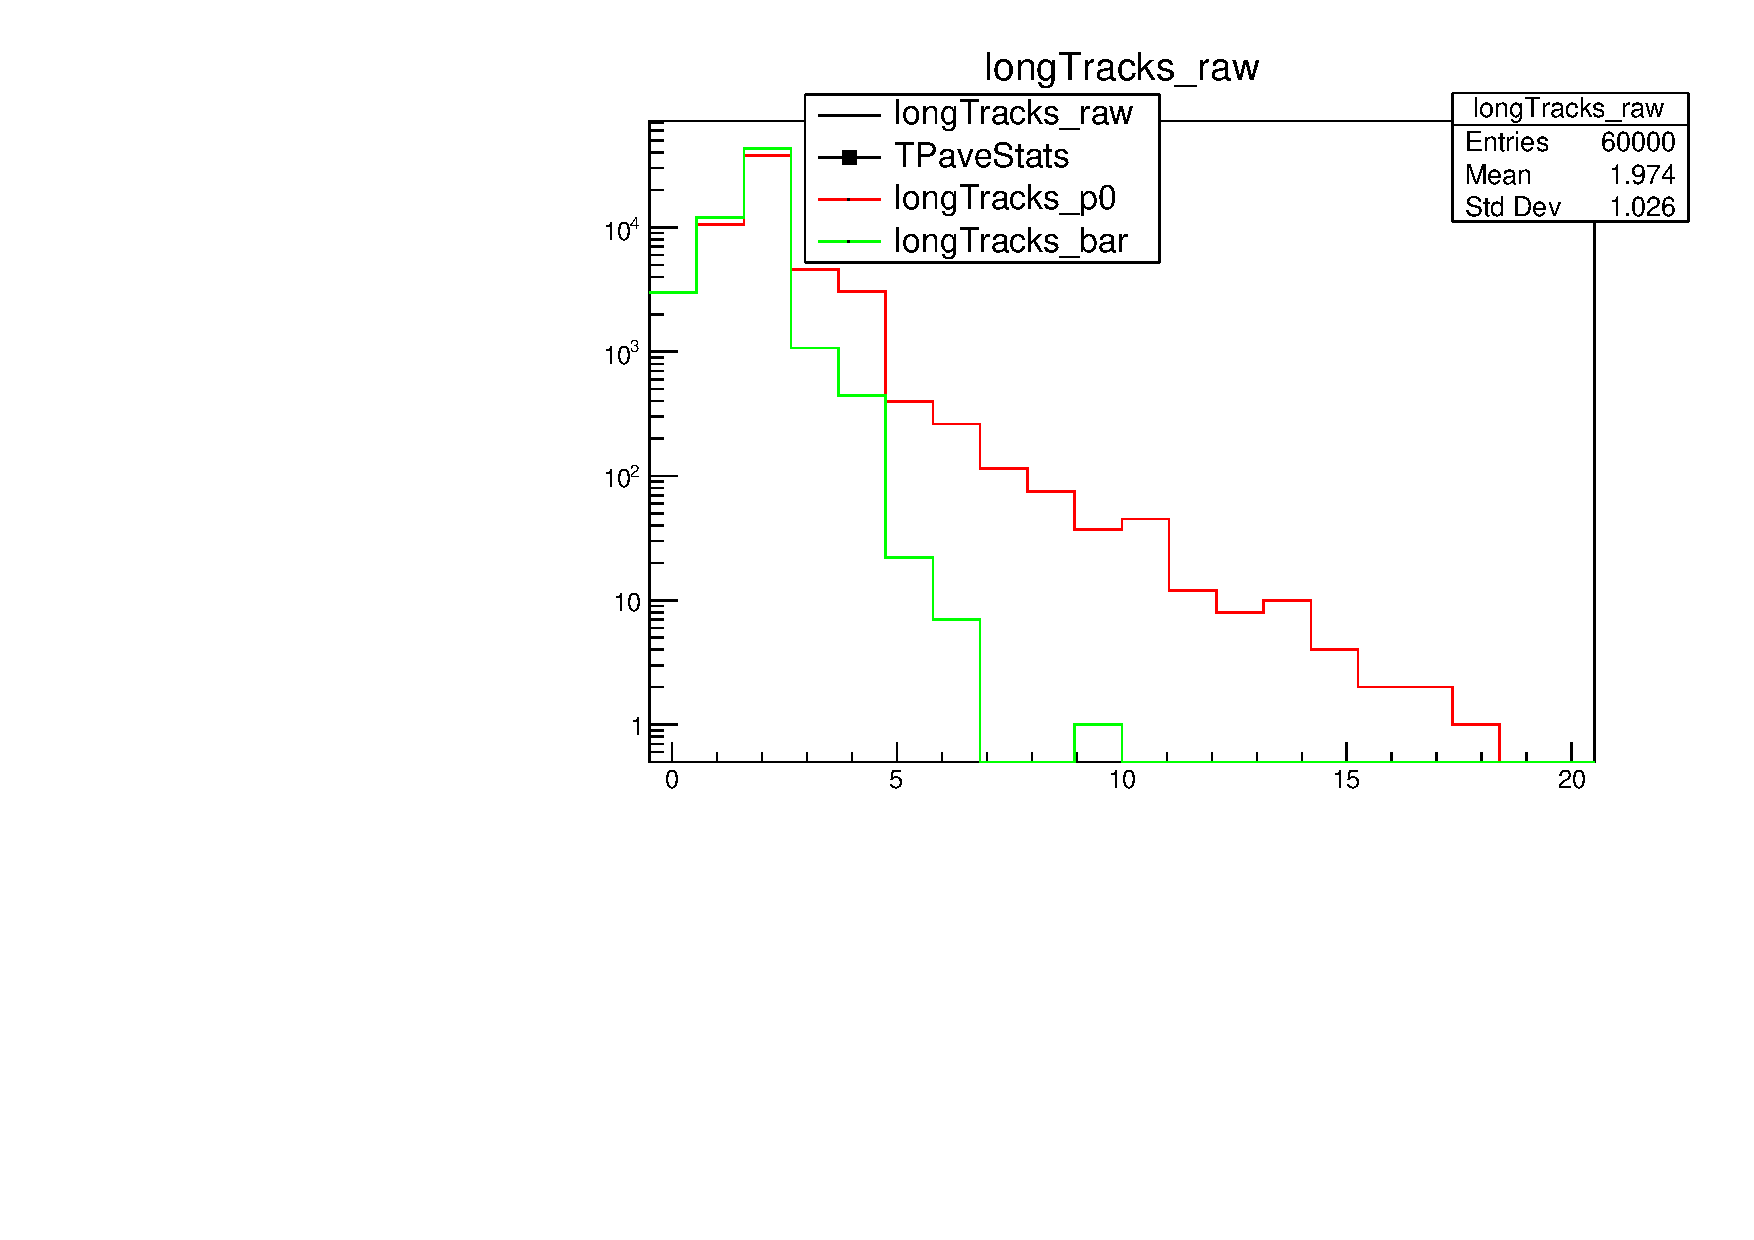
\includegraphics[width=1\linewidth]{assets/longTracksCompared_al9.pdf}
%     \end{figure}
% \end{frame}
% \begin{frame}{Why do the Efficiencies decay at Station 1?}
%     \begin{itemize}
%         \item The efficiency is not increasing with separation
%     \end{itemize}
%     \begin{figure}
%         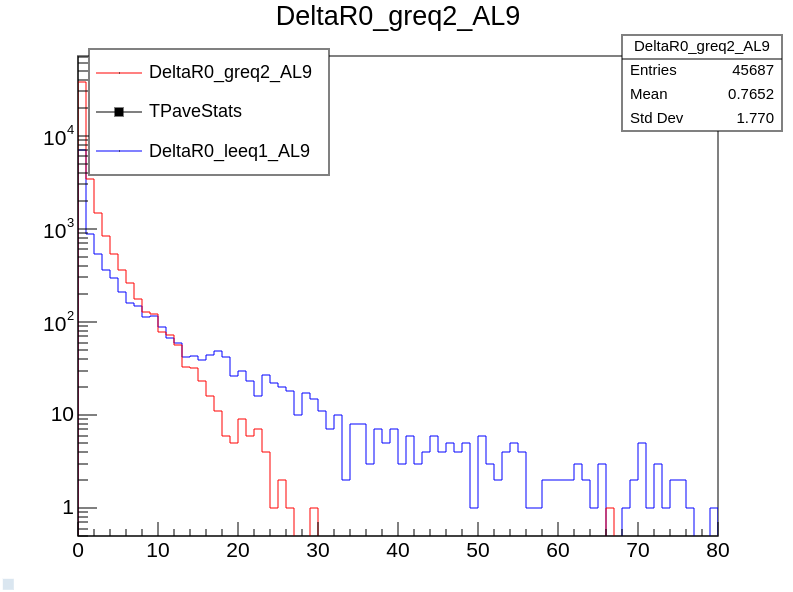
\includegraphics[width=0.7\linewidth]{assets/gr2vsle1.png}
%     \end{figure}
%     \begin{itemize}
%         \item $\geq$2 tracks aren't being reconstructed ``better'' with separation
%         \item Even then $\leq$1 track events are being reconstructed ``better''
%     \end{itemize}
% \end{frame}

% \section{Dark Photon CutFlow from Ansh's Study [SKIP]}
% \includepdf[pages={3-5}]{assets/Alma9vsCentos7Efficiencies.pdf}

